\chapter{Clustering and Overfitting Analysis}

\section{The Data Leakage Problem}
In many audio datasets, multiple segments are recorded from the same machine in a single session. These segments are highly correlated. If a standard random split is used, segments from the same session appear in both the training and test sets. 

The model effectively "memorizes" the unique background hum or specific microphone noise of that session and uses it to identify the machine, rather than learning generalizable fault indicators. This leads to artificially high accuracy scores (~99\%) that vanish when the model is tested on truly new machinery.

\section{Intra-Class Clustering Strategy}
To solve this, we implemented a clustering-aware splitting strategy. By grouping similar recordings within each class using K-Means, we created "Acoustic Groups."

\subsection{K-Means Clustering}
For each of the six classes, we run K-Means on the acoustic feature vectors. Each sample is assigned a Cluster ID. During cross-validation, we use \texttt{GroupKFold}, ensuring that all samples from a specific cluster are either entirely in the training set or entirely in the validation set.

\begin{figure}[H]
    \centering
    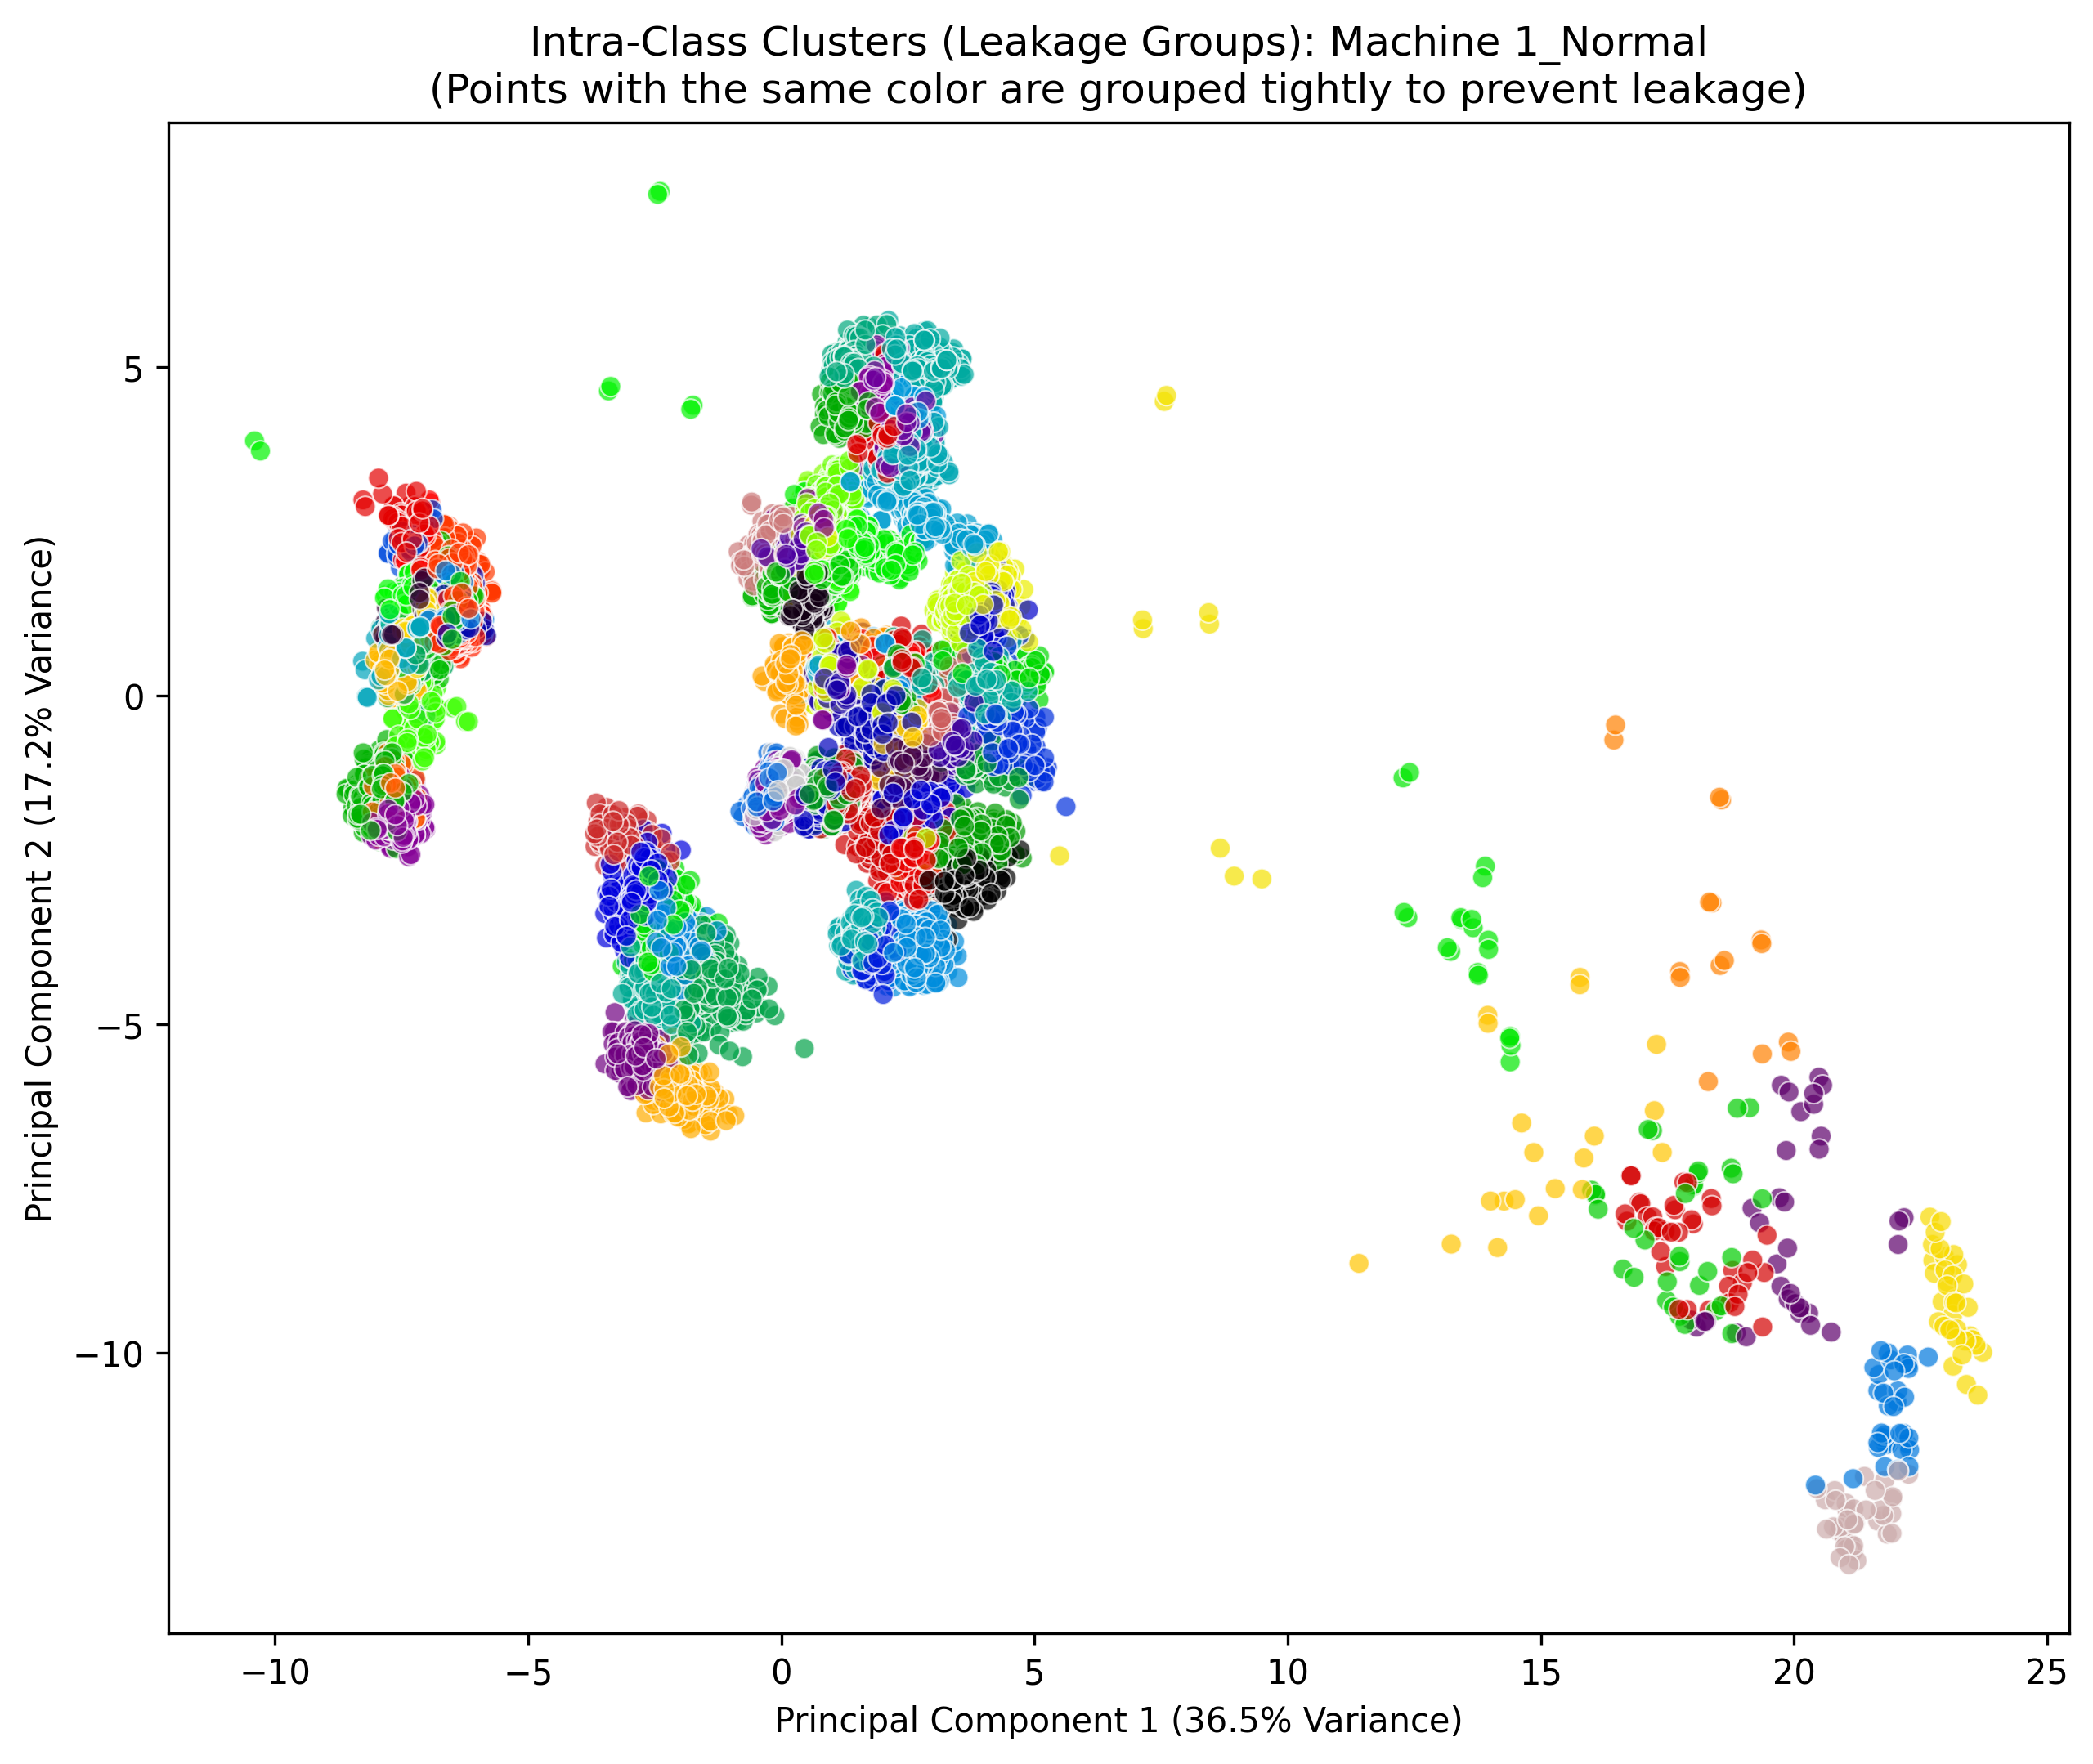
\includegraphics[width=0.8\textwidth]{figures/cluster_Machine_1_Normal.png}
    \caption{Visualizing Intra-Class K-Means Clustering for Machine 1 Normal}
    \label{fig:kmeans_cluster}
\end{figure}

\section{Optimizing Cluster Granularity}
The number of clusters (granularity) is the most critical hyperparameter for preventing leakage.

\subsection{Comparison of Runs}
We conducted an empirical study to find the "Goldilocks" zone of clustering:
\begin{table}[H]
    \centering
    \caption{Granularity Analysis and Performance}
    \begin{tabular}{@{}lccc@{}}
        \toprule
        \textbf{Samples/Cluster} & \textbf{CV F1-Score} & \textbf{Test F1-Score} & \textbf{Outcome} \\ \midrule
        10 (Run 3) & 0.98 & 0.99 & Over-granular (Leakage) \\
        60 (Run 2) & 0.96 & 0.98 & Moderate Leakage \\
        300 (Run 4) & \textbf{0.89} & \textbf{0.92} & \textbf{Optimized Baseline} \\
        1000 (Run 1) & 0.49 & 0.76 & Under-granular (Underfitting) \\ \bottomrule
    \end{tabular}
\end{table}

\subsection{Selection of 300 Samples per Cluster}
By targeting 300 samples per cluster, we ensure that the clusters are large enough to encompass entire recording sessions, thus preventing the model from learning file-specific signatures. This results in a slightly lower but far more realistic performance metric, which reflects the model's true ability to generalize to new machines.

\section{Unsupervised Session Discovery (DBSCAN)}
As an alternative approach for the Deep Learning pipeline, we utilized DBSCAN (Density-Based Spatial Clustering of Applications with Noise). This method is particularly effective for discovering the "physical recording events" that constitute the dataset without relying on class labels.

\subsection{Feature Representation for Discovery}
To provide DBSCAN with a rich acoustic context, we extracted a 232-dimensional feature vector for every file. This vector includes:
\begin{itemize}
    \item \textbf{MFCCs (120 dims):} Mean, std, and delta-mean per coefficient.
    \item \textbf{Spectral Features (8 dims):} Centroid, bandwidth, rolloff, and flatness (mean and std).
    \item \textbf{Chroma and Tonnetz (36 dims):} Capturing harmonic relationships and pitch classes.
    \item \textbf{Mel-Spectrogram Stats (64 dims):} Energy distribution across 32 Mel bands.
\end{itemize}

\subsection{Dimensionality Reduction Pipeline}
The high-dimensional feature space was compressed to facilitate density-based clustering:
\begin{enumerate}
    \item \textbf{StandardScaler:} Normalizing features to zero mean and unit variance.
    \item \textbf{PCA:} Retaining 95\% of the variance to remove noise and redundant correlations.
    \item \textbf{UMAP (15-D):} Projecting the data into a 15-dimensional manifold specifically tuned for DBSCAN distance metrics (\texttt{n\_neighbors=30}, \texttt{min\_dist=0.0}).
\end{enumerate}

\begin{figure}[H]
    \centering
    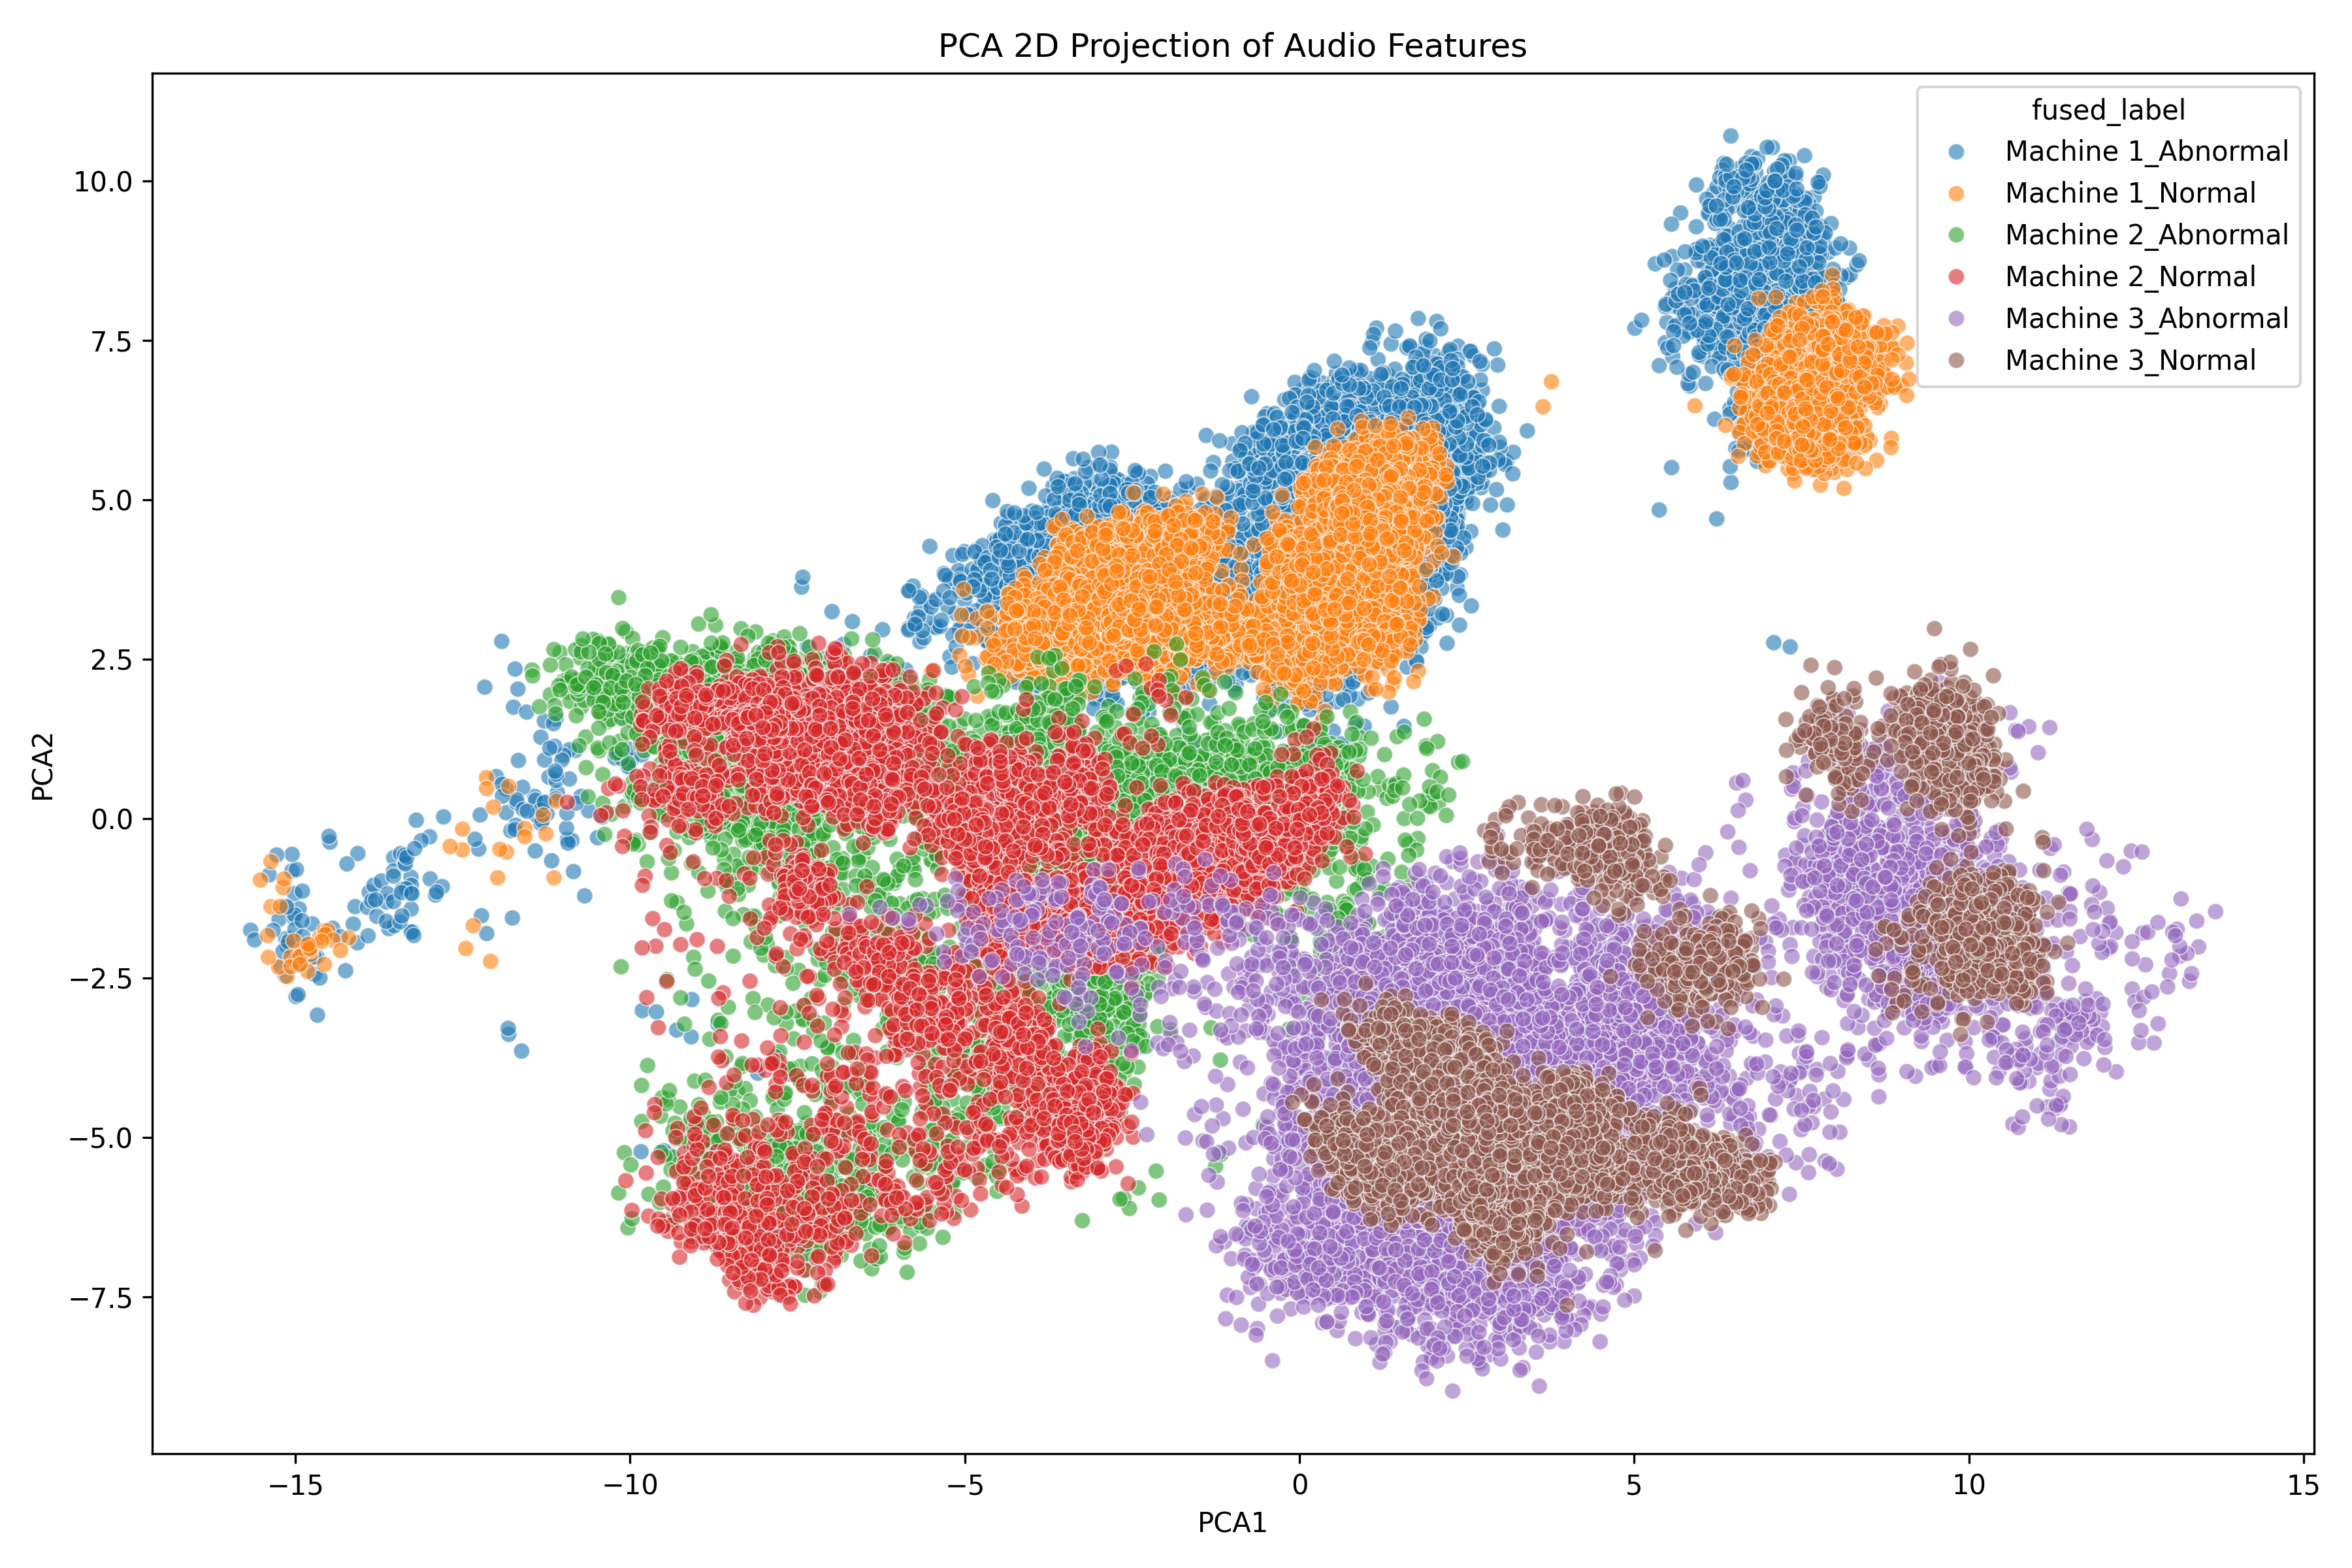
\includegraphics[width=0.8\textwidth]{figures/pca_plot.png}
    \caption{PCA Cumulative Variance Analysis for Feature Compression}
    \label{fig:pca_plot}
\end{figure}

\subsection{Clustering Performance Metrics}
The DBSCAN parameters ($eps$ and $min\_samples$) were optimized using a grid search validated by unsupervised metrics:
\begin{itemize}
    \item \textbf{Silhouette Score:} Measuring how similar an object is to its own cluster compared to others.
    \item \textbf{Davies-Bouldin Index:} Evaluating the ratio of within-cluster distances to between-cluster distances.
    \item \textbf{Adjusted Rand Index (ARI):} Comparing the discovered clusters against true session labels (when available) to ensure physical relevance.
\end{itemize}

This process successfully identified distinct clusters representing unique recording environments, which were subsequently used to define the groups for our leak-free data splits.
